\documentclass{article}

\usepackage[utf8]{inputenc}  % For encoding support
\usepackage{amsmath}         % For mathematical formatting
\usepackage{graphicx}        % For including images
\usepackage{xcolor}
\usepackage[a4paper, left=0.5in, right=0.5in, top=0.5in, bottom=0.5in]{geometry}  % Adjust margins here

\title{Parallel Programming Notes}
\author{Ayush Raina}
\date{\today}

\begin{document}

\maketitle

\section*{Lecture 1: Architectures 1}
\subsection*{Classification of Architectures - Flynns Classification}
\begin{itemize}
    \item SISD: Single Instruction Single Data, for example, serial computers.
    \item SIMD: Single Instruction Multiple Data, for example, vector processors and processor arrays.
    \item MISD: Multiple Instruction Single Data, for example, trying different ways to decrypt a message.
    \item MIMD: Multiple Instruction Multiple Data, for example, multi-core processors.
\end{itemize}

\subsection*{Classification based on Memory}
\begin{itemize}
    \item \textbf{Shared Memory:} All processors share a common memory. Communication is done using this shared address space. This is further classified into UMA (Uniform Memory Access) and NUMA (Non-Uniform Memory Access).
    \begin{itemize}
        \item UMA: All processors have equal access time to all memory locations. Memory access is slow and has limited bandwidth. UMA has single memory controller.
        \item NUMA: Processors have variable access to memory locations. Memory access is faster and has higher bandwidth than UMA. NUMA has multiple memory controllers.
    \end{itemize}
    \item \textbf{Distributed Memory:} Each processor has its own memory. 
\end{itemize}

Shared memory could itself be distributed among processor nodes. Each processor might have some portion of the memory that is physically close to it and therefore accessible in less time.

\subsection*{Cache Coherence Problem}
If each processor in a shared memory multiprocessor machine has a data cache, then the problem of cache coherence arises. Our objective is that processes should not read \textcolor{blue}{\textbf{stale}} data.

\subsection*{Cache Coherence Protocols}
\begin{itemize}
    \item \textbf{Write Invalidate:} When a processor writes to its cache, it sends invalidate signal to all other caches that have a copy of that memory location. This means all other cache locations must discard their copy of the memory location and fetch it again from the main memory if needed.
    \item \textbf{Write Update:} When a processor writes to its cache, it sends the updated data to other caches that have a copy of that memory location. This keeps all caches up to date.
\end{itemize}

\subsection*{False Sharing}
If two processors access different variables that are located within same cache line but are not related to each other. In this case any write to one variable will cause cache line to be invalidated and other processor might have to reload the data from main memory. This is called false sharing.

In next lecture we will discuss about interconnecting networks.
\newpage

\section*{Lecture 2: Architectures 2}
\subsection*{Interconnection Networks}

They are used in both shared memory to connect processors to memory and in distributed memory to connect different processors to each other. Components for interconenction networks are interfaces such as Peripheral Component Interconnect (PCI) or PCI - Express used for connecting processors to network and a network link which connected to communication network.

\subsection*{Communication Network}
It consists of switching elements to which processors are connected through ports. \textbf{Switching elements} receive data from one point and send it to another point. \textbf{Switch} refers to collection of these switching elements. \textbf{Network topology} is specific pattern of connections in which these switching elements are connected. \\
In shared memory systems processors as well as memory units are connected to communication network. 

\subsection*{Different Kinds of Network Topologies}
1. \textbf{Bus:} All processors are connected to a single bus. It is simple and cheap but has limited bandwidth. \\
2. \textbf{Crossbar Switch:} It consists of 2D grid of switching elements, where each switching element consists of two input and two output ports. Input Ports are connected to output ports through a switching logic. \\

In previous case of Crossbar Switch, we require $nm$ switching elements where $n$ is number of processors and $m$ is number of memory units in case of shared memory architecture or $m$ is the number of processors in distributed memory architectures. To reduce switching complexity, we can use \textbf{Multistage Network - Omega Network}. \\

3. \textbf{Omega Network:} It consists of $log P$ stages each consisting of $P/2$ switching elements. \\

Consider Distributed Memory Architecture. In Crossbar switch, there is dedicated path for any processor to communicate with any other processor without contention but in Omega Network, there is contention if 2 processors wants to communicate to 2 different processors, they might have to take same path through some stage of the network. \\

If $P_i$ and $P_j$ wants to communicate in Omega Network, first convert $ID(P_i)$ and $ID(P_j)$ to binary and then keep comparing most significant bits and follow \textbf{cut through routing} or \textbf{pass through routing} to reach destination. \\

Some commonly used network topologies used in distributed memory architectures are Mesh, Torus, hypercubes and Fat tree. \\

1. \textbf{Mesh:} Grid of switching elements where each switching element is connected to 4 directional neighbours. \\
2. \textbf{Torus:} Mesh with wrap around connections. In this $T(i,1)$ is connected to $T(i,n) \forall i$. Similarly $T(1,j)$ is connected to $T(m,j) \forall j$. \\ 
3. \textbf{Hypercube:} Keep Joining binary n cubes to get hypercube. In hypercubes, distance between any two processors is bit difference between their binary representation. \\
4. \textbf{Fat Tree:} It is a tree like structure where each node is a switch and each switch has multiple ports. Leaves are processors. As we go up the tree, number of ports in switch increases. This is Non Blocking Network means no contention because there is unique path between any two processors. Fat Tree has a special property which makes all this happen and that is \textbf{Number of Links from node to a children = Number of Links from node to parent}. \\

\textbf{bandwidth: } maximum amount of data that can be transferred over the network in given time, usually measured in bits per second. (bps) 

\newpage

\subsection*{Evaluating Interconnection Topologies}
1. \textbf{Diameter: } Maximum distance between any two processing nodes.Smaller diameter means lower latencies. \\
2. \textbf{Connectivity: } Number of Paths between two nodes. It can also be defined as minimum number of links that need to be removed to disconnect the network. Higher connectivity improves fault tolerance.\\
3. \textbf{Fault Tolerance: } Ability of network to operate correctly even if some links or switches fail. \\
4. \textbf{Bisection Width: } Minimum number of links that need to be removed to divide the network into two equal halves. \\
5. \textbf{Channel Width: } Number of bits that can be simultaneously communicated over a link i.e number of physical wires between two nodes. Higher Channel width increases data transfer capacity. \\
6. \textbf{Channel Rate: } Performance of single physical wire i.e The speed at which single physical wire transmits the data and is generally measured in bits per second(bps). \\
7. \textbf{Channel bandwidth: } The total data transfer capacity of a link. It is calculated as Channel Width * Channel Rate. Higher Channel bandwidth allows faster communication. \\
8. \textbf{Bisection bandwidth: } This is defined as maximum volume of communication between two halves of network or in other words maximum data transfer capacity between two halves of network and is given by bisection width * channel bandwidth. Higher bisection bandwidth means better performance under heavy traffic. \\

\subsection*{Questions / Doubts }
1. How fat tree network has constant bisection bandwidth? \\

\newpage

\section*{Lecture 3: Parallelization Principles}
We have seen several advantages of parallelism, but there are also some overheads which are not seen in sequential programs like \textbf{communication delay}, \textbf{synchronization} and \textbf{idling}.

\begin{figure}[h]
    \centering
    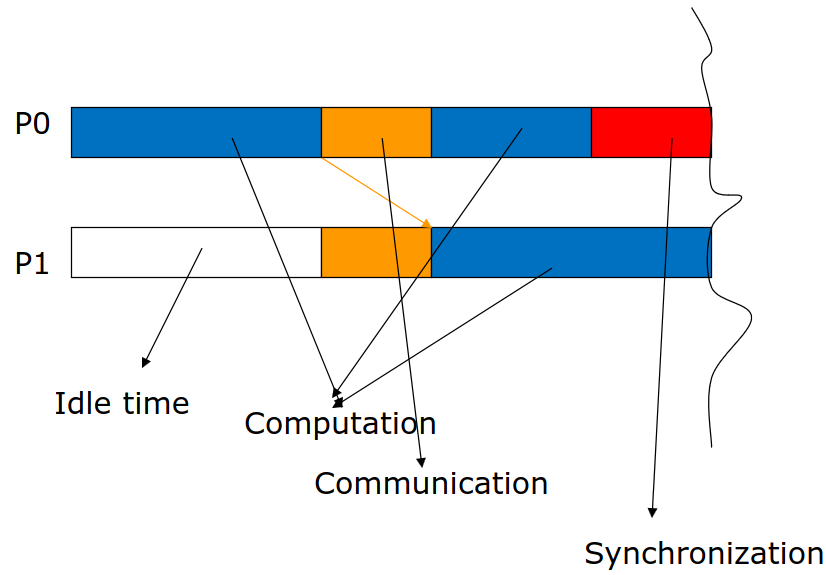
\includegraphics[width=0.5\textwidth]{overheads.png}
    \caption{Overheads}
\end{figure}

\subsection*{Evaluation of Parallel Program}
Let us denote execution time by $T_p$ for parallel program using $p$ processors. \\

1. \textbf{Speedup:} $S(p,n) = T(1,n) / T(p,n)$ where $T(1,n)$ is execution time of sequential program. Usually $S(p,n) \leq p$ as we expect program to get $p$ times faster in idead case but sometimes $S(p,n) > p$ which is called \textbf{superlinear speedup}. Ideally we want $S(p,n) = p$. \\

2. \textbf{Efficiency:} $E(p,n) = S(p,n) / p$. Efficiency is a measure of how well the parallel program is utilizing the resources. Generally $E(p,n) \leq 1$, but in case of superlinear speedup, $E(p,n) > 1$. Ideally we want $E(p,n) = 1$. \\

3. \textbf{Cost:} $C(p,n) = T(p,n) * p$. It is similar to Efficiency but relates the runtime to number of utilized processors. \\

4. \textbf{Scalability:} We want to measure the efficieny of parallel program for variable number of processors. This is called scalability analysis. There are two types of scalability - \textbf{Strong Scalability} and \textbf{Weak Scalability}. In strong scalability, we measure the efficiencies for varying number of processors while keeping indut data size fixed. In weak scalability, we measure efficiency of parallel code by varying both the number of processors and input data size. \\

We will now derive an upper bound on achievable speedup when parallelizing a given sequential program. Let $T_{seq}$ and $T_{par}$ denote the parts whihc cannot benefit from parallelization and can benefit from parallelization respectively. Further assume we can get ideal linear speed up and super linear speedup is also possible. Then we have $T(p,n) \geq T_{seq} + T_{par} / p$. \\

The Speedup is given by \[\Large \boxed{S(p,n) = \frac{T(1,n)}{T(p,n)} \leq \frac{T_{seq} + T_{par}}{T_{seq} + T_{par} / p}}\] 
Instead of using the actual runtimes, now use fraction of the total runtime. Let $f$ be such that $T_{seq} = f * T(1,n)$ and $T_{par} = (1-f) * T(1,n)$. Then we have \[\Large \boxed{S(p,n) \leq \frac{1}{f + \frac{1-f}{p}}}\]

The above equation is known as Amdahl's Law. Now we can see some examples: \\
\begin{enumerate}
    
    \item Suppose 95\% of a rogram’s execution time occurs inside a loop that we want to parallelize. What is the maximum speedup we can expect from a parallel version of our program executed on six processors?
\end{enumerate}

\[\Large \boxed{S(6,n) \leq \frac{1}{0.05 + \frac{0.95}{6}} = 4.8} \]

\begin{enumerate}
    \setcounter{enumi}{1}
    \item 10\% of the program's execution time is spent within sequential code. What is limit to speedup achievable by parallel version ?
\end{enumerate}

Since we are not given how many processors are used, we assume ideal case of unbounded processors.
\[\Large \boxed{ S(\infty,n) \leq \lim_{p \to \infty} \frac{1}{0.1 + \frac{0.9}{p}} = 10} \]

We can see the limitation to Amdahl's Law is that it only applies in situation where problem size is fixed. We will now derive a more general upper bound on speedup. Let $\alpha$ be the scaling function for the sequential part of program and $\beta$ be the scaling function for the parallel part of program. Both $\alpha$ and $\beta$ are w.r.t to complexity of problem size. \\
This means $T_{seq}$ grows as $\alpha * T(1,n)$ as problem size grows and $T_{par}$ grows as $\beta * T(1,n)$ as problem size grows. \\

\[ T_{\alpha \beta} (1,n) = \alpha * T_{seq} + \beta * T_{par} = \alpha * f * T(1,n) + \beta * (1-f) * T(1,n) \]
\[ T_{\alpha \beta} (p,n) = \alpha * T_{seq} + \frac{\beta * T_{par}}{p} = \alpha * f * T(1,n) + \frac{\beta * (1-f) * T(1,n)}{p} \]

Then we have \[\Large \boxed{S_{\alpha \beta}(p,n) \leq \frac{\alpha * f + \beta * (1-f)}{\alpha * f + \frac{\beta * (1-f)}{p}}}\]

Let $\gamma = \frac{\beta}{\alpha}$, then we have \[\Large \boxed{S_{\gamma}(p,n) \leq \frac{f + \gamma * (1-f)}{f + \frac{\gamma * (1-f)}{p}}}\]

Now depending on the value of $\gamma$, we can have different upper bounds on speedup. 
\begin{enumerate}
    \item Amdahl's Law: $\gamma = 1$ which means $\alpha = \beta$
    \item Gustafson's Law: $\gamma = p$ which means $\alpha=1$ and $\beta=p$. This means parallel part of program grows linearly in $p$ as problem size grows. In this case the formula becomes \[\Large \boxed{S(p,n) \leq f + (1-f) * p}\]
    
    This law can also be thought as by knowing f , we can use it to predict the
    theoretically achievable speedup using multiple processors when parallelizable part scales linearly with the problem size while the serial part remains constant
\end{enumerate}

let us discuss some examples: \\
\begin{enumerate}
    \item Suppose we have a parallel program that is 15\% serial and 85\% linearly parallelizable for a given problem size. Assume that the (absolute) serial time does not grow as the problem size is scaled.\\
    
    (i) How much speedup can we achieve if we use 50 processors without scaling the problem - $S_{\gamma=1}(50,n)$
    (ii) Suppose we scale up the problem size by a factor of 100. How much speedup could we achieve with 50 processors - $S_{\gamma=100}(50,n)$
\end{enumerate}

\subsection*{Roofline Performance Model}
This gives a bound on the performance of an application on a particular architecture and it also helps to categorize the code's performance as memory bound or performance bound. It depends on three parameters - Peak Performance of the machine $P_{peak} \;\; (FLOP/s)$, Memory Bandwidth $B_{peak} \;\; (Bytes/s)$ and Computational Intensity $I_{op} \;\; (FLOP/Byte)$. \\

\subsection*{Questions / Doubts}
1. Discuss this Roofline Model again with Professor and work out some examples. \\

\section*{Lecture 4.1: Parallel Programming Models}
Some parallel programming models include Single Program Multiple Data (SPMD) and Multiple Program Multiple Data (MPMD). We will focus on SPMD model. \\

\subsection*{Programming Paradigms}
\begin{enumerate}
    \item Shared Memory Model: Threads, Open MP, CUDA.
    \item Distributed Memory Model: MPI - Message Passing Interface.
\end{enumerate}

\subsection*{Data Parallelism and Domain Decomposition}
Given data is divided into processing entities. Each process owns and computes a portion of the data.\\
Multidimensional Data in simulations is divided into subdomains and each subdomain is assigned to a processing entity. This is called \textbf{Domain Decomposition}. 

\subsection*{Process Grids} 
Given P processors are arranged in multi dimensions forming a process grid. Once this is done then domain of problem is divided in process grid.

\subsection*{Distribution of Data}
There are various ways of distributing data like block distribution, cyclic distribution, block cyclic distribution etc. Check Parallelization Principles pdf in good notes for visualization.

\section*{Lecture 4.2: PRAM Model}
PRAM Stands for Parallel Random Access Machine. Helps to write precursor (initial version) parallel algorithms without any architecture constraints. Allows algorithm designers to treat processing power as unlimited and it ignores complexity of inter communication.

\subsection*{Benefits of PRAM Model}
\begin{enumerate}
    \item Helps in designing parallel algorithms as PRAM provides a basic structure that can be adapted to real world parallel machines.
    \item Base PRAM algorithm can help establish tight lower and upper bounds for practical implementations and assumptions made in PRAM model helps architecture designers for improving their designs.
    \item Can be suitable for modern day architectures like GPU's.
\end{enumerate}

\newpage

\subsection*{PRAM Model Architecture}
The PRAM can be viewed as an ideal shared memory architecture that does not consider any overheads. . Thus, when designing PRAM algorithms we can focus on the best possible parallel algorithm design. Asymptotic runtimes of optimal PRAM algorithms can often be 
taken as lower bounds for implementations on actual machines.

\begin{figure}[h]
    \centering
    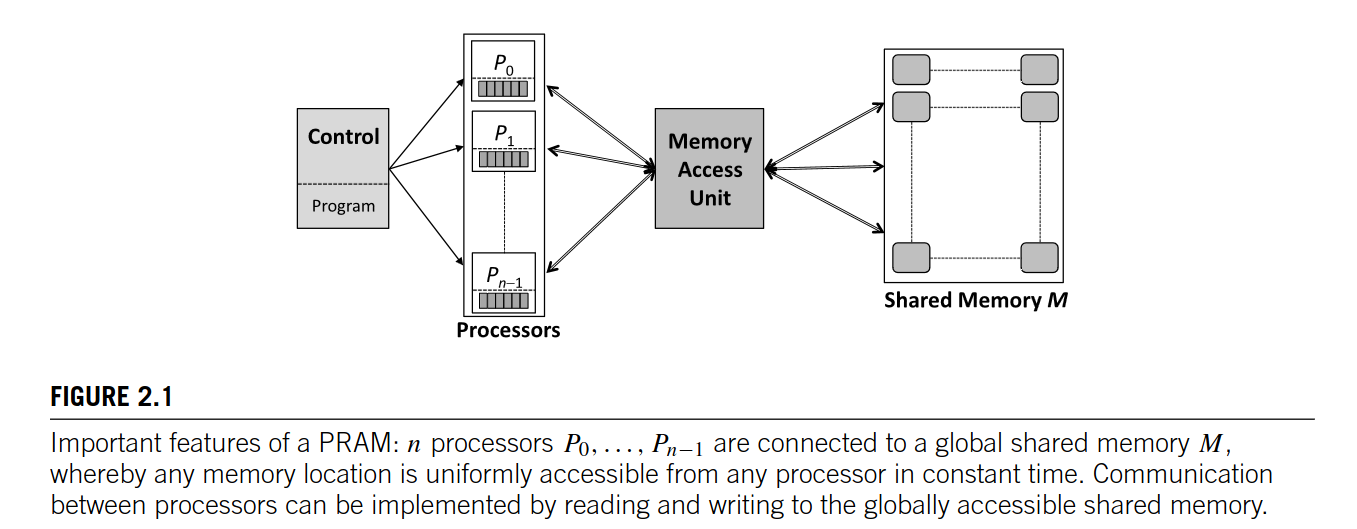
\includegraphics[width=0.9\textwidth]{Images/PRAM.png}
    \caption{PRAM Model}
\end{figure}

PRAM consists of $n$ identical processors $P_i$ for $0 \leq i \leq n-1$. In every step each processor executes an instruction cycle in three phases:
\begin{enumerate}
    \item \textbf{Read Phase:} Each processor can simultaneously read a single data item from a (distinct) shared memory cell and store it in a local register.
    \item \textbf{Compute Phase:} Each processor can perform a fundamental operation on its local data and subsequently stores the result in a register.
    \item \textbf{Write Phase:} Each processor can simultaneously write a data item to a shared memory cell,whereby the exclusive write PRAM variant allows writing only distinct cells while concurrent write PRAM variant also allows processors to write to the same location which can lead to race conditions.
\end{enumerate} 

Three phase PRAM instructions are executed synchronously. Communications between the processors in the PRAM needs to be implemented in terms of reading and writing to shared memory. This type of memory can be accessed in a uniform way; i.e., each processor has access to any memory location in unit (constant) time. This makes it more powerful than real shared memory machines in which accesses to (a large) shared memory is usually non-uniform and much slower compared to performing computation on registers. The PRAM can therefore be regarded as an idealized model of a shared memory machine; e.g. we cannot expect that a solution for a real parallel machine is more efficient
than an optimal PRAM algorithm.

\subsection*{PRAM Variants}
Several types of PRAM variants have been defined which differ in how data in shared memory can be read/written: only exclusively or concurrently. So we have 4 possible combinations
\textbf{ER} - Exclusive Read, \textbf{CR} - Concurrent Read, \textbf{EW} - Exclusive Write, \textbf{CW} - Concurrent Write. These are also shown in Figure 2.2.
We now describe three most popular variants the EREW, CREW, and CRCW PRAMs.

\begin{figure}[h]
    \centering
    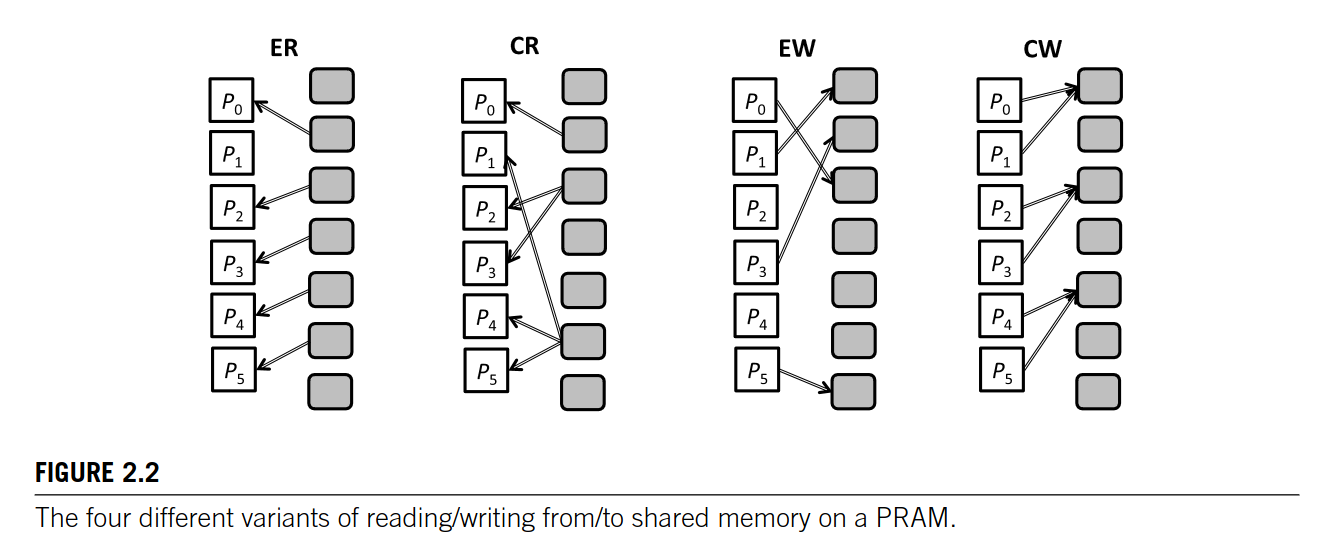
\includegraphics[width=0.9\textwidth]{Images/PRAM2.png}
    \caption{PRAM Variants}
\end{figure}

\subsection*{EREW PRAM}
EREW stands for Exclusive Read Exclusive Write. No two processors are allowed to read or write to the same memory location during same cycle.

\subsection*{CREW PRAM}
CREW stands for Concurrent Read Exclusive Write. Several processors may read data from the same shared memory cell simultaneously. Still, different processors are not allowed to write to the same shared memory cell.

\subsection*{CRCW PRAM}
CRCW stands for Concurrent Read Concurrent Write. Both simultaneous reads and writes to the same shared memory cell are allowed in this variant. In case of a simultaneous write (analogous to a race condition) we need to further specify which value will actually be stored. \\

There are 4 common approaches to deal with the situation where two or more processors attempt to write to same memory location during the same clock cycle are:
\begin{enumerate}
    \item Priority Concurrent Write (CW) - Processors have been assigned distinct priorities and the processor with the highest priority succeeds in writing its value to the shared memory.
    \item Arbitary Concurrent Write (CW) - A randomly choosen processor succeeds in writing its value to the shared memory.
    \item Common Concurrent Write (CW) - All processors writing to same global memory must write the same value.
    \item Combining Concurrent Write (CW) - All values to be written are combined into a single value by means of an associative binary operations such as sum, product, minimum, or logical AND.
\end{enumerate}

\subsection*{Parallel Prefix Sum Computation}
1. First method involves spawnning N threads and each thread computes one element of the prefix sum array. Here is simple CUDA kernel code for this one assuming that threads are distributed in such a way global thread ID $\leq N-1$.

\begin{figure}[h]
    \centering
    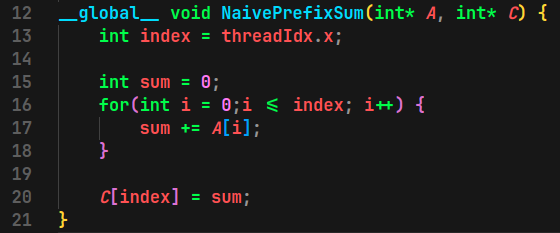
\includegraphics[width=0.6\textwidth]{Images/prefix1.png}
    \caption{Prefix Sum CUDA Kernel $\mathcal{O}(n^2)$}
\end{figure}

2. Second method is slightly better approach than first one and is easy to understand from followig figure

\begin{figure}[h]
    \centering
    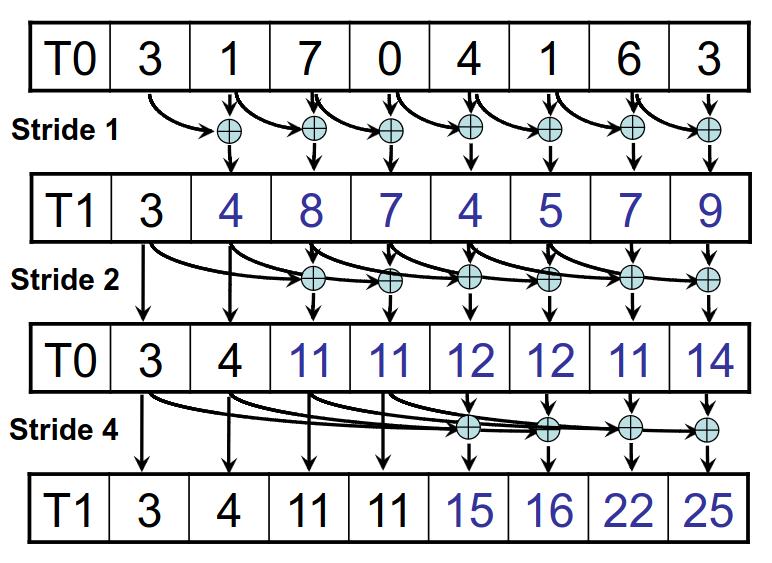
\includegraphics[width=0.6\textwidth]{Images/prefix2method.png}
    \caption{Prefix Sum Approach 2 $\mathcal{O}(nlogn)$}
\end{figure}

Here is the CUDA kernel code for this method.

\begin{figure}[h]
    \centering
    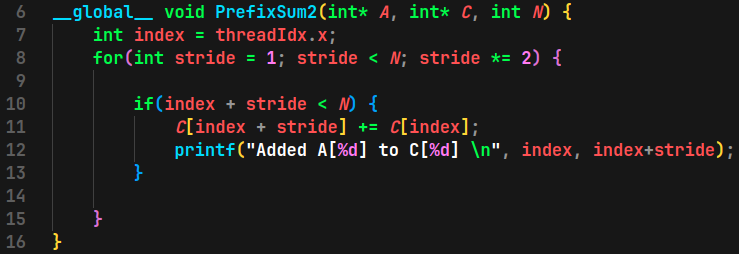
\includegraphics[width=0.8\textwidth]{Images/prefix2.png}
    \caption{Prefix Sum CUDA Kernel}
\end{figure}

\newpage
\subsection*{Parallel Merge of 2 Sorted Lists}
Normally merge of two sorted lists takes $\mathcal{O}(m+n)$ time and $\mathcal{O}(m+n)$ space. Where as if we have to do this in constant space then it will take $\mathcal{O}(mlogm + nlogn)$ time, Here in our parallel algorithm we will have $n$ processors for $n$ elements in first list and $m$ processors for $m$ elements in second list.

\begin{itemize}
    \item The processor knows index of element in own list.
    \item It then finds the index of element in other list using binary search.
    \item sum of these two indices gives the index of element in merged list.
    \item Write the element to this index in merged list.
\end{itemize}

Clearly we can see that the complexity is $\mathcal{O}(nlogm + mlogn)$. Here is the CUDA kernel code for this algorithm. This algorithm will only work if all elements in both lists are \textbf{distinct}.

\begin{figure}
    \centering
    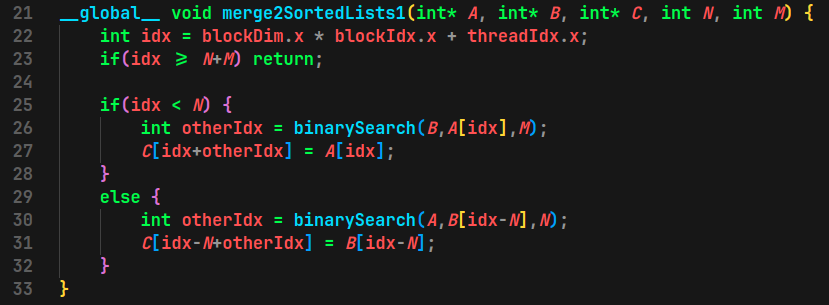
\includegraphics[width=0.6\textwidth]{Images/mergeList1.png}
    \caption{Merge of 2 Sorted Lists CUDA Kernel}
\end{figure}

\begin{figure}
    \centering
    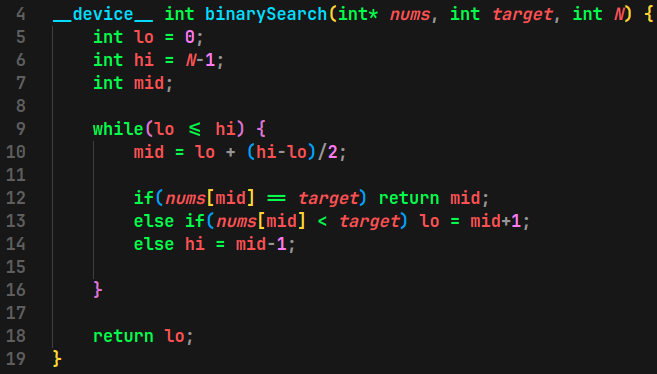
\includegraphics[width=0.6\textwidth]{Images/binarySearch.png}
    \caption{Device Function for Binary Search}
\end{figure}

\newpage

\subsection*{Enumeration Sort}

\end{document}
